\documentclass[12pt]{article}


\usepackage[T1]{fontenc}
\usepackage[polish]{babel}
\usepackage[utf8]{inputenc}
\usepackage{lmodern}
\selectlanguage{polish}
\usepackage{graphicx}

\title{Styczna do wykresu funkcji}
\date{}
\begin{document}
\maketitle
\noindent
Niech funkcja \textit{f} będzie określona w otoczeniu \textit{U}($x_{0}$) oraz niech będzie różniczkowalna w samym punkcie $x_0$. Ponadto niech \textit{h} będzie liczbą rzeczywistą, dla której ($x_0$+\textit{h}) $\in$ \textit{U}($x_{0}$). Rozważmy \textit{P}$\left(x_0, f(x_0)\right)$ oraz \textit{Q}$\left(x_0+h, f(x_0+h)\right)$ należące do wykresu funkcji \textit{f}. Przez te punkty prowadzimy prostą (rysunek poniżej przedstawia przypadek \textit{h}>0).\\
\begin{equation}
\label{tw1}
[f(x)+g(x)]'= f'(x)+g'(x) 
\end{equation}
\begin{equation}
\label{tw2}
[f(x)-g(x)]'= f'(x)-g'(x) 
\end{equation}
\\
Wzoru (\ref{tw1}) będziemy używać do obliczania pochodnej sumy funkcji.\\
Zaś do obliczania pochodnej różnicy funkcji będziemy używać wzoru (\ref{tw2}).
\begin{figure}[ht]
\begin{center}
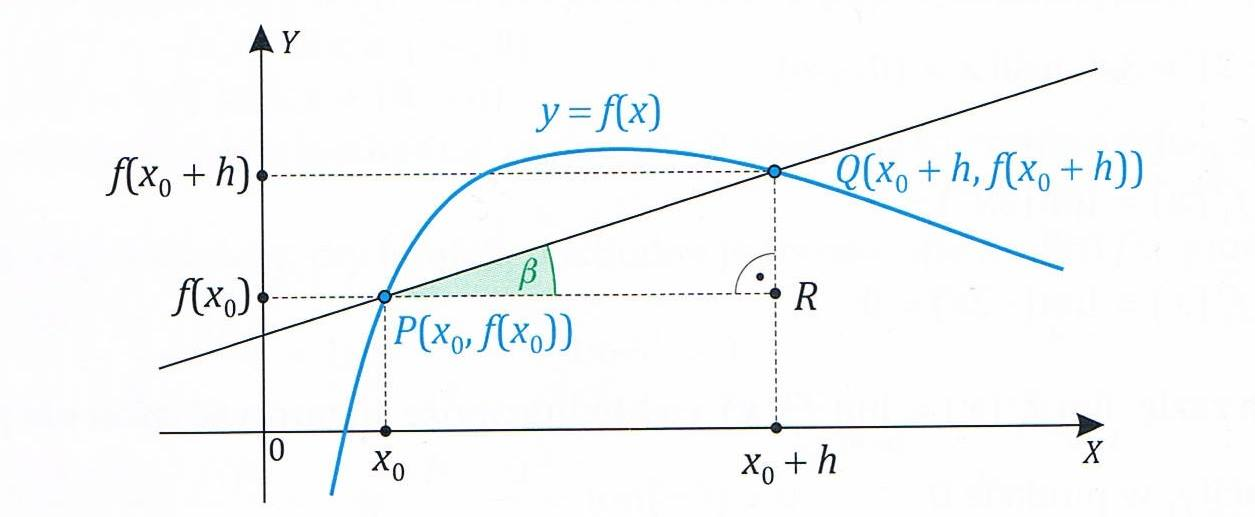
\includegraphics[height=3cm]{zdj1.jpg}
\caption{Rysunek omawianej funkcji}
\label{rys_model}
\end{center}
\end{figure}\\
Taką prostą nazywamy sieczną wykresu funkcji \textit{f}, przechodzącą przez punkty \textit{P,Q}.\\
 Oznaczmy miarę kąta \textit{RPQ} przez $\beta$. Wyznaczamy tg$\beta$:\\ 
 \begin{equation}
 \label{twierdzenie}
 tg \beta = \frac{f(x_0+h)-f(x_0)}{h}
 \end{equation}
\newpage Okazuje się, że iloraz różnicowy funkcji \textit{f} w punkcie $x_0$, odpowiadający zmianie argumentu \textit{h}, jest współczynnikiem kierunkowym rozważanej siecznej.\\
\\
Zobaczmy, co się będzie działo, jeżeli \textit{h} będzie dążyć do 0. Wówczas punkt \textit{Q} będzie ,,coraz bliżej'' punktu \textit{P}. 
\begin{figure}[ht]
\begin{center}
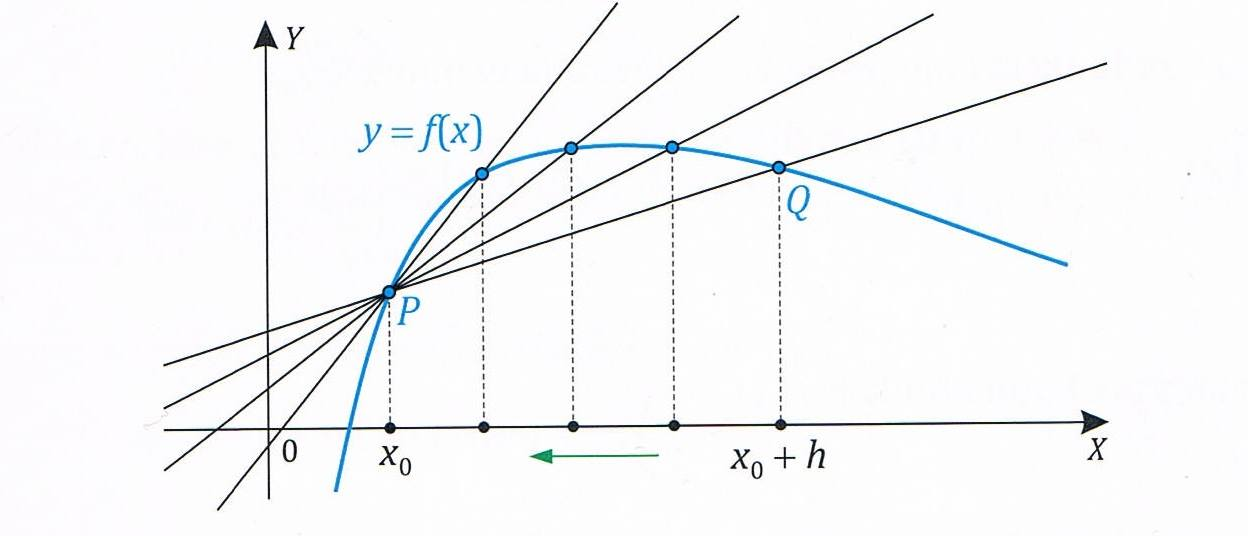
\includegraphics[height=3cm]{zdj2.jpg}
\caption{Ilustracja \textit{h} dążącego do 0}
\label{rys2_model}
\end{center}
\end{figure}
\begin{center}
Podstawowe wzory na pochodne funkcji:
\end{center}
\[
\begin{array}{c|c|c}
funkcja & pochodna \hspace{5px} funkcji & dziedzina  \hspace{5px} pochodnej\\
\hline
f(x)=c & f'(c)= 0 & R \\
f(x) = ax + b & f'(x) = a & R\\
f(x) = ax^2 + bx + c & f'(x) = 2ax + b & R
\end{array}
\]
\end{document}